\section{Auswertung}
\label{sec:Auswertung}

Zunächst wird der Brechungsindex für die parallele sowie die senkrechte
Polarisation berechnet. Dazu werden die Fresnelschen Formeln nach dem 
Brechungsindex $n$ umgestellt. Die Messwerte Der gemessenen Lichtintensität $I_\text{r}$
bei dem Winkel $\alpha$ sind \autoref{tab:10}  zu entnehmen. Die Berechnungen der Brechungsindizes 
finden in zwei unterabschnitten \autoref{sec:10} und \autoref{sec:11} statt und die Ergebnisse sind 
dann gemeinsam in \autoref{tab:11} zu finden. Für die Rechnungen wird die Intensität zu $I = \frac{I_r}{I_e}$ 
benutzt, wobei $I_e = 0.255\unit{\milli\ampere}$  Die gemessene intensität des einfallenden Lichts beschreibt.
Der Dunkelstron $I_d$ wird als vernachlässigbar klein angenommen, da das Messgerät in der Größenordnung keine 
Verlässlichen Werte anzeigt.

\begin{table}[H]
  \centering
  \caption{Messwerte der Lichtreflexion}
  \label{tab:10}
  \begin{tblr}{
          colspec = {S S S S | S S S S},
          row{1} = {guard, mode = math},
          row{2} = {guard, mode = math},
      }
      \toprule
       \SetCell[c=4]{c} \text{Parallel} & & & & \SetCell[c=4]{c} \text{Senkrecht} & \\
      \alpha \, /\unit{\degree}& I \, /\unit{\milli\ampere}& \alpha \, /\unit{\degree} & I \, /\unit{\milli\ampere}&\alpha \, /\unit{\degree}& I \, /\unit{\milli\ampere}& \alpha \, /\unit{\degree} & I \, /\unit{\milli\ampere}\\
      \midrule
      85  &0.1400 &  53 & 0.0120  &  87 & 0.500 &  35 & 0.016\\
      83  &0.0900 &  51 & 0.0100  &  85 & 0.480 &  33 & 0.012\\
      82  &0.0680 &  49 & 0.0100  &  83 & 0.460 &  31 & 0.012\\
      81  &0.0440 &  47 & 0.0120  &  81 & 0.460 &  29 & 0.012\\
      80  &0.0280 &  45 & 0.0100  &  79 & 0.410 &  27 & 0.010\\
      79  &0.0180 &  43 & 0.0100  &  77 & 0.400 &  25 & 0.012\\
      78  &0.0120 &  41 & 0.0120  &  75 & 0.360 &  23 & 0.010\\
      77  &0.0074 &  39 & 0.0140  &  73 & 0.320 &  21 & 0.012\\
      76  &0.0042 &  37 & 0.0120  &  71 & 0.280 &  19 & 0.012\\
      75  &0.0030 &  35 & 0.0100  &  69 & 0.220 &  17 & 0.010 \\
      74  &0.0032 &  33 & 0.0080  &  67 & 0.200 &  15 & 0.010\\
      73  &0.0040 &  31 & 0.0100  &  65 & 0.180 &  13 & 0.010\\
      72  &0.0052 &  29 & 0.0100  &  63 & 0.120 &  11 & 0.010\\
      71  &0.0072 &  27 & 0.0120  &  61 & 0.100 &  9  & 0.010\\
      70  &0.0090 &  25 & 0.0100  &  59 & 0.100 &  7  & 0.010\\
      69  &0.0100 &  23 & 0.0100  &  57 & 0.072 &  5  & 0.010\\
      68  &0.0120 &  21 & 0.0100  &  55 & 0.060 &  3  & 0.010\\
      67  &0.0140 &  19 & 0.0100  &  53 & 0.040 &     &  \\
      66  &0.0160 &  17 & 0.0100  &  51 & 0.038 &     &  \\
      65  &0.0160 &  15 & 0.0120  &  49 & 0.030 &     &   \\
      64  &0.0160 &  13 & 0.0100  &  47 & 0.026 &     &  \\
      63  &0.0180 &  11 & 0.0100  &  45 & 0.022 &     &  \\
      61  &0.0180 &  9  & 0.0100  &  43 & 0.018 &     &  \\
      59  &0.0180 &  7  & 0.0100  &  41 & 0.016 &     &  \\
      57  &0.0180 &  5  & 0.0100  &  39 & 0.018 &     &  \\
      55  &0.0140 &          &     &  37 & 0.018 &     &  \\
      \bottomrule 
  \end{tblr}
\end{table}
Die Werte des Senkrecht polarisierten lichts sind bis $\alpha = 31\unit{\degree}$ mit einem Fehler von 
$\Delta I = \qty{0.02}{\milli\ampere}$ und ab $\alpha = 33\unit{\degree}$ mit einem Fehler von 
$\Delta I = \qty{0.002}{\milli\ampere}$ versehen. Die Messwerte der reflektierten Intensität
des Parallel polarisierten Lichts sind bis $\alpha = 12\unit{\degree}$ mit $\Delta I = \qty{0.02}{\milli\ampere}$ versehen, 
zwischen $\alpha = 13\unit{\degree}$ und $\alpha = 20\unit{\degree}$ mit $\Delta I = \qty{0.002}{\milli\ampere}$ und ab 
$\alpha = 13\unit{\degree}$ sind die Werte wieder mit einem Fehler von $\Delta I = \qty{0.02}{\milli\ampere}$ versehen.

\begin{table}[H]
  \centering
  \caption{Berechnete Brechungsindizes}
  \label{tab:11}
  \begin{tblr}{
          colspec = {S S S S | S S S S},
          row{1} = {guard, mode = math},
          row{2} = {guard, mode = math},
      }
      \toprule
       \SetCell[c=4]{c} Parallel & & & & \SetCell[c=4]{c} Senkrecht & \\
      \alpha \, /\unit{\degree}& n & \alpha \, /\unit{\degree} & n&\alpha \, /\unit{\degree}& n& \alpha \, /\unit{\degree} & n\\
      \midrule
      85  &12.6+-0.5 & 53 &  1.35+-0.12 &  87 & 1.5+-0.5&  35 &   1.3+-0.6\\
      83  &8.66+-0.35&  51 & 1.26+-0.13 &  85 & 1.8+-0.6&  33 &   1.2+-0.7\\
      82  &7.45+-0.30&  49 & 1.18+-0.15 &  83 & 2.0+-0.7&  31 &   1.2+-0.7\\
      81  &6.51+-0.27&  47 & 1.12+-0.18 &  81 & 2.4+-0.9&  29 &   1.3+-0.8\\
      80  &5.78+-0.24&  45 & 1.06+-0.21 &  79 & 2.2+-0.6&  27 &   1.2+-0.8\\
      79  &5.21+-0.22&  43 & 1.04+-0.18 &  77 & 2.4+-0.7&  25 &   1.3+-0.8\\
      78  &4.74+-0.20&  41 & 1.03+-0.13 &  75 & 2.2+-0.6&  23 &   1.3+-0.9\\
      77  &4.35+-0.18&  39 & 1.03+-0.10 &  73 & 2.1+-0.5&  21 &   1.3+-0.9\\
      76  &4.02+-0.17&  37 & 1.02+-0.09 &  71 & 1.9+-0.4&  19 &   1.3+-0.9\\
      75  &3.74+-0.16&  35 & 1.01+-0.08 &  69 & 1.71+-0.31&  17 & 1.3+-0.9\\
      74  &3.50+-0.15&  33 & 1.01+-0.07 &  67 & 1.71+-0.31&  15 & 1.3+-1.0\\
      73  &3.28+-0.14&  31 & 1.01+-0.06 &  65 & 1.69+-0.31&  13 & 1.3+-1.0\\
      72  &3.09+-0.14&  29 & 1.01+-0.06 &  63 & 1.48+-0.26&  11 & 1.3+-1.0\\
      71  &2.92+-0.13&  27 & 1.01+-0.05 &  61 & 1.44+-0.26&  9  & 1.3+-1.0\\
      70  &2.77+-0.13&  25 & 1.01+-0.05 &  59 & 1.49+-0.29&  7  & 1.3+-1.0\\
      69  &2.63+-0.12&  23 & 1.01+-0.05 &  57 & 1.40+-0.29&  5  & 1.3+-1.0\\
      68  &2.50+-0.12&  21 & 1.01+-0.05 &  55 & 1.37+-0.31&  3  & 1.3+-1.0\\
      67  &2.38+-0.12&  19 & 1.01+-0.05 &  53 & 1.29+-0.33&     &  \\
      66  &2.28+-0.11&  17 & 1.01+-0.04 &  51 & 1.31+-0.35&     &  \\
      65  &2.17+-0.11&  15 & 1.01+-0.04 &  49 & 1.3+-0.4&     &   \\
      64  &2.08+-0.11&  13 & 1.01+-0.04 &  47 & 1.3+-0.4&     &  \\
      63  &1.99+-0.11&  11 & 1.01+-0.04 &  45 & 1.3+-0.5&     &  \\
      61  &1.84+-0.10&  9  & 1.01+-0.04 &  43 & 1.2+-0.5&     &  \\
      59  &1.70+-0.10&  7  & 1.01+-0.04 &  41 & 1.2+-0.6&     &  \\
      57  &1.57+-0.10&  5  & 1.01+-0.04 &  39 & 1.3+-0.6&     &  \\
      55  &1.45+-0.11&      &         &  37&1.3+-0.6& &  \\
      \bottomrule 
  \end{tblr}
\end{table}

(toolbox) ju
\subsection{Paralleler Brechungsindex}
\label{sec:10}
Die Fresnel Formel für Parallele polarisation ergibt umgestellt nach $n$
\begin{equation}
n = \sqrt{\frac{E}{2\cdot\cos{\alpha}^2} + \sqrt{\frac{E^2}{4\cdot\cos{\alpha}^4} - E \cdot \tan{\alpha}^2}}
\end{equation}
Dabei ist $E = \frac{(I+1)^2}{(I - 1)^2}$ für $\alpha < \alpha_\text{brewster}$ und  
$E = \frac{(I-1)^2}{(I + 1)^2}$ für $\alpha > \alpha_\text{brewster}$. 
Durch Mittelung der Ergebnisse aus\autoref{tab:11} beläuft sich der Mittlere Wert auf 
\begin{equation}
  \overline{n_\text{parallel}} = \qty{2.50(0.32)}{}
\end{equation}

\subsection{Senkrechte Polarisation}
\label{sec:11}
Bei der Senkrechten polarisaton ergibt sich $n$ zu
\begin{equation}
n = \sqrt{1+\frac{4\cdot E \cos{\alpha}^2}{(E-1)^2}}  , E = \sqrt{I}
\end{equation}
Damit ergibt sich mit den Werten der Senkrechten brechungsindizes in \autoref{tab:11} 
\begin{equation}
 \overline{n_\text{senkrecht}} = \qty{1.48(0.05)}{}
\end{equation}
\subsection{Theorievergleich mit den Messswerten}
Um die gemessenen Intensitäten mit den Theoriewerten zu vergleichen, sind 
diese in \autoref{fig:10} zusammen mit den Theoriekurven abgebildet. 
\begin{figure}[H]
  \centering 
  \caption{Messswerte und theoriekurve}
  \label{fig:10}
  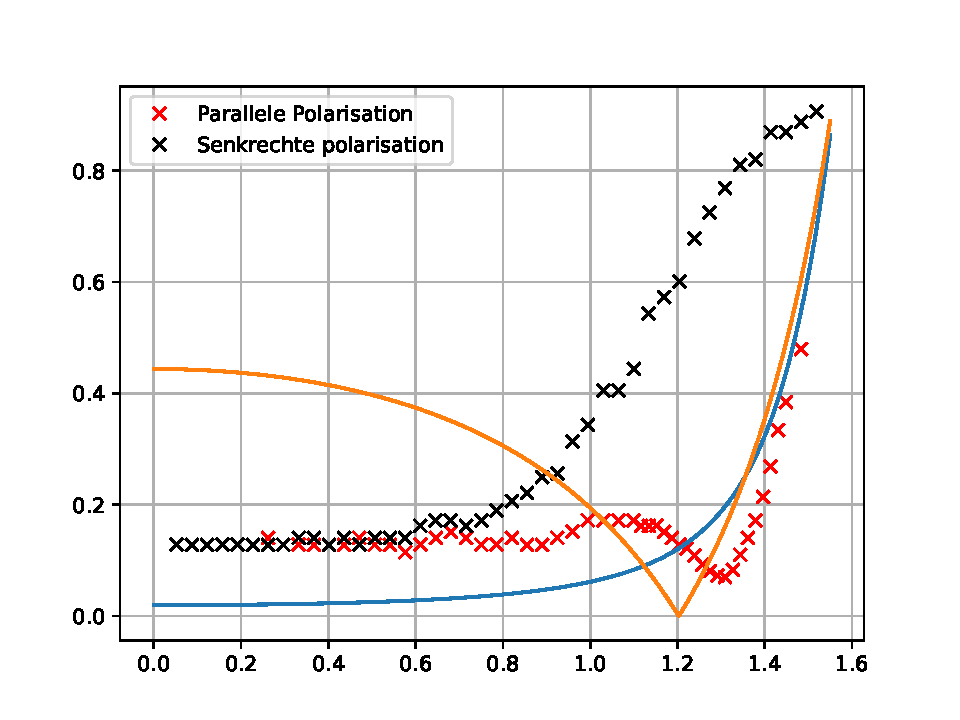
\includegraphics{build/plot.pdf}
\end{figure}
\subsection{Brewster Winkel}
Den Gemessenen intensitäten bei Paralleler polarisationsrichtung in \autoref{tab:10} kan man entnehmen, dass 
der Brewster Winkel zwischen $\alpha = \qty{73}{\degree}$ und $\alpha = \qty{74}{\degree}$ liegen müsste. Mit dem 
gemittelten Brechungsindex bei paralleler Polarisationsrichtung $n_\text{parallel} = \qty{2.50(0.32)}{}$ ergibt sich nach \autoref{eqn:8}
ein Brewster Winkel von
\begin{equation}
 \theta_\text{Brewster} = \qty{68.17}{\degree}
\end{equation}
Aus dem aus unseren Messdaten abgelesenen Brewster Winkel $\Theta_\text{Brewster}=75\unit{\degree}$ ergibt sich 
ein Brechungsindex von  
\begin{equation}
 n_\text{Brewster} = \qty{0.96}{}
\end{equation}
